\chapter{Remaining useful life: Turbofan engines}


\section{Data}

\begin{remark}
    Maintenance can be of three types:
    \begin{descriptionlist}
        \item[Reactive maintenance]
            Repair when something is broken.

        \item[Preventive maintenance]
            Periodically change something, in a conservative way, before it breaks.

        \item[Predictive maintenance]
            Change when something is close to break.
    \end{descriptionlist}

    Remaining useful life (RUL) is a metric useful for predictive maintenance.
\end{remark}

The dataset contains run-to-failure experiments on NASA turbofan engines. Excluding domain specific features, the main columns are:
\begin{descriptionlist}
    \item[\texttt{machine}] Index of the experiment.
    \item[\texttt{cycle}] Time step of the experiment.
    \item[\texttt{rul}] Remaining useful life.
\end{descriptionlist}


From the dataset heatmap, the following can be observed:
\begin{itemize}
    \item Rows with a uniform blue or red color represent features that contain frequent short-lived variations (i.e., peeks) that skew the standard deviation.
    \item Some features show a trend synced with the experiments (see rows around 15 at the y-axis with blue peeks at the end of each experiment).
\end{itemize}
\begin{figure}[H]
    \centering
    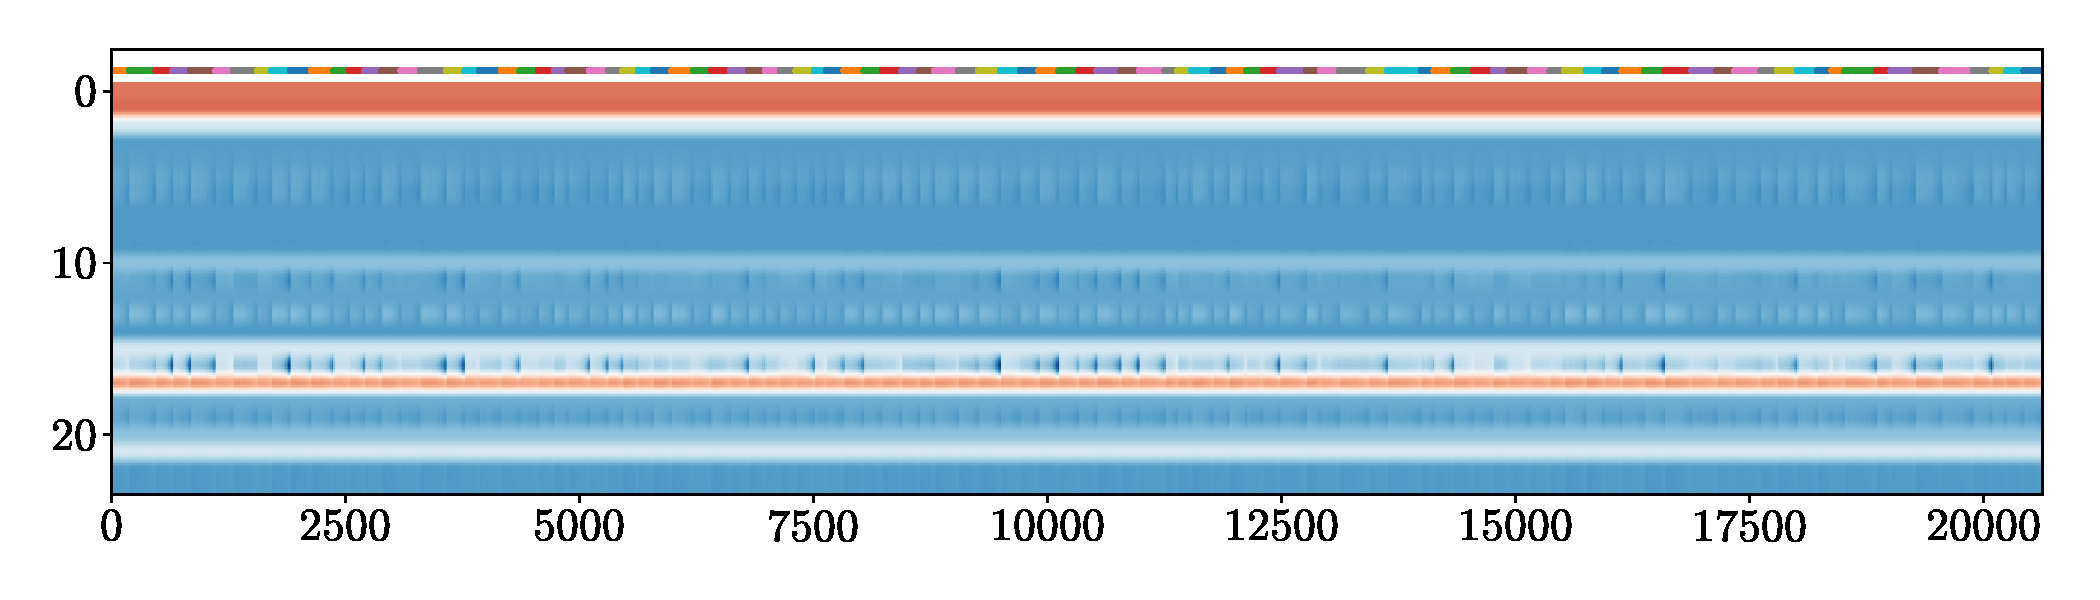
\includegraphics[width=0.95\linewidth]{./img/_rul_heatmap.pdf}
    \caption{
        \parbox[t]{0.7\linewidth}{
            Heatmap of the dataset. On the top line, each section represents an experiment.
        }
    }
\end{figure}


\subsection{Data splitting}

As the dataset is composed of experiments, standard random sampling will mix experiments and leak information. Therefore, sampling is done on the experiments in chronological order (train first).

\begin{remark}
    When splitting, the train data should be representative of the test data. Moreover, the test set should be representative of the real world.
\end{remark}


\section{Approaches}


\subsection{Regressor}

Predict RUL with a regressor $f$ and set a threshold to trigger maintenance:
\[ f(x, \theta) \leq \varepsilon \]